\section{Профиль и протокол}
\subsection{Цель и основные соотношения}
Цель --- разделить влияние расписания шума, ошибки сети и численной схемы генерации~\cite{teacher}. При $\alpha_t=1-\beta_t$, $\bar\alpha_t=\prod_{s=1}^t\alpha_s$, $\bar\alpha_0=1$ прямой процесс вычисляется за один шаг:
\begin{equation}x_t=\sqrt{\bar\alpha_t}x_0+\sqrt{1-\bar\alpha_t}\,\epsilon,\quad \epsilon\sim N(0,I),\quad SNR(t)=\frac{\bar\alpha_t}{1-\bar\alpha_t}.\end{equation}
Линейное расписание интерполирует beta между границами. Косинусное использует $f(t)=\cos^2((t/T+0.008)\pi/(2\cdot1.008))$; после ограничения $\beta_t\le0.999$ произведение $\bar\alpha$ пересчитано. Ядро расписания использует float64.

Сеть предсказывает epsilon; loss --- средний квадрат ошибки по объектам и координатам. Поэтому численные $L_{simple}$ приведены на координату; запись нормы без деления на $d=2$ увеличила бы их вдвое, не меняя обучения. Из предсказания получаются
\begin{equation}\hat x_0=\frac{x_t-\sqrt{1-\bar\alpha_t}\,\epsilon_\theta}{\sqrt{\bar\alpha_t}},\qquad s_\theta=-\frac{\epsilon_\theta}{\sqrt{1-\bar\alpha_t}}.\end{equation}
Оптимальный предиктор равен $\epsilon_*=E[\epsilon|x_t]$, а не реализованному шуму. Для смеси гауссиан точная плотность после зашумления остаётся смесью с центрами $\sqrt{\bar\alpha_t}\mu_m$ и ковариациями $\bar\alpha_t\Sigma_m+(1-\bar\alpha_t)I$. Score $s_*=\nabla\log p_t$ вычислен стабильно, через log-sum-exp в стандартизованных координатах.

DDPM проходит все $T$ шагов с $\mu_\theta=\alpha_t^{-1/2}(x_t-\beta_t\epsilon_\theta/\sqrt{1-\bar\alpha_t})$ и posterior variance $\tilde\beta_t=\beta_t(1-\bar\alpha_{t-1})/(1-\bar\alpha_t)$. Последний шаг не добавляет шум, clipping выключен. DDIM использует $\tau_i=\operatorname{round}(iT/K)$; при $\eta=0$
\begin{equation}x_{\tau_{i-1}}=\sqrt{\bar\alpha_{\tau_{i-1}}}\hat x_0+\sqrt{1-\bar\alpha_{\tau_{i-1}}}\hat\epsilon_i.\end{equation}
Последний шаг возвращает $\hat x_0$. При полной сетке и $\eta=1$ DDIM совпадает с DDPM. Здесь $\eta$ --- случайность DDIM, не шаг Ланжевена.

\subsection{Данные, сеть и метрики}
Профиль: $T=1000$, $\beta\in[0.0001,0.02]$, $M=6$, $\rho=0.1$, $\pi_0=0.02$. Центры $\mu_m=(\cos(2\pi m/6),\sin(2\pi m/6))$, ковариация $0.01I$. Мода 0 редкая; прочие веса равны 0.196. Train/val/test 20 000/5000/5000, seeds 701/702/703; cal не используется.

Статистики рассчитаны только по train:
\begin{equation}\mu=(-0.18077255,0.00254579),\quad s=(0.62488898,0.77288930).\end{equation} Преобразование по координатам $z=(x-\mu)/s$, обратное $x=z\odot s+\mu$. Модель и точный score работают в $z$, качество считается в исходных единицах.

MLP: вход 2, шесть скрытых слоёв ширины 256, SiLU, синусоидальное вложение времени 128 с отдельным MLP. Преобразованное время вводится в каждый скрытый слой. Adam 0.001, batch 512, 20 000 обновлений; RTX 3060 Laptop, float32, без AMP и TF32. При сравнении расписаний архитектура и все остальные условия одинаковы.

Каждая оценка использует 5000 генерируемых точек и фиксированный test. Частоты цели оценены на 100 000 новых точках, seed 704; внешняя категория включает расстояния не меньше $3\rho$. $Cov$ сравнивает частоту каждой моды с половиной её справочной частоты; $D_{mode}$ --- полная вариация по шести модам и внешней категории. RBF MMD$^2$ --- V-статистика с фиксированной медианной полосой $h=1.23793506$ по всем парам train. Пять свежих истинных выборок задают шум метрик. Фиксированные значения: MMD2 noise mean = 0.00012093903, MMD2 noise sd = 4.1371986e-05, Dmode noise mean = 0.009434, Dmode noise sd = 0.0019972431.

\section{E1. Расписания шума}
Теоретическое ожидание: оба расписания стирают конечный сигнал, но различно распределяют сложность по времени. Доля шагов SNR$<0.01$ равна 0.326 у linear и 0.064 у cosine. Конечный условный KL усреднён по train:
\begin{equation}\overline{KL}_T=\frac12\overline{\bar\alpha_T\|x_0\|^2-d\bar\alpha_T-d\ln(1-\bar\alpha_T)}.\end{equation}
\begin{table}[H]\centering\scriptsize
\setlength{\tabcolsep}{4pt}
\caption{E1: единственное различие обучения --- расписание шума; DDPM, 5000 точек.}\label{tab:e1}
\begin{tabular}{lrrrrrrl}
\toprule
Расписание & $\bar\alpha_T$ & KL & Train loss & Val loss & MMD$^2$ & $D_{mode}$ & Ист. \\
\midrule
linear & 4.036e-05 & 4.036e-05 & 0.40611 & 0.40820 & 0.0021705 & 0.05625 & R01 \\
cosine & 2.429e-09 & 2.429e-09 & 0.69308 & 0.68686 & 0.0021917 & 0.05185 & R02 \\
\bottomrule
\end{tabular}
\end{table}


Оба $\bar\alpha_T$ ниже $10^{-3}$. Cov обеих моделей равен 1. Более низкий linear loss не даёт однозначного превосходства двух метрик качества: разница MMD$^2=-0.000021205$, Dmode=+0.00440.
\begin{figure}[H]\centering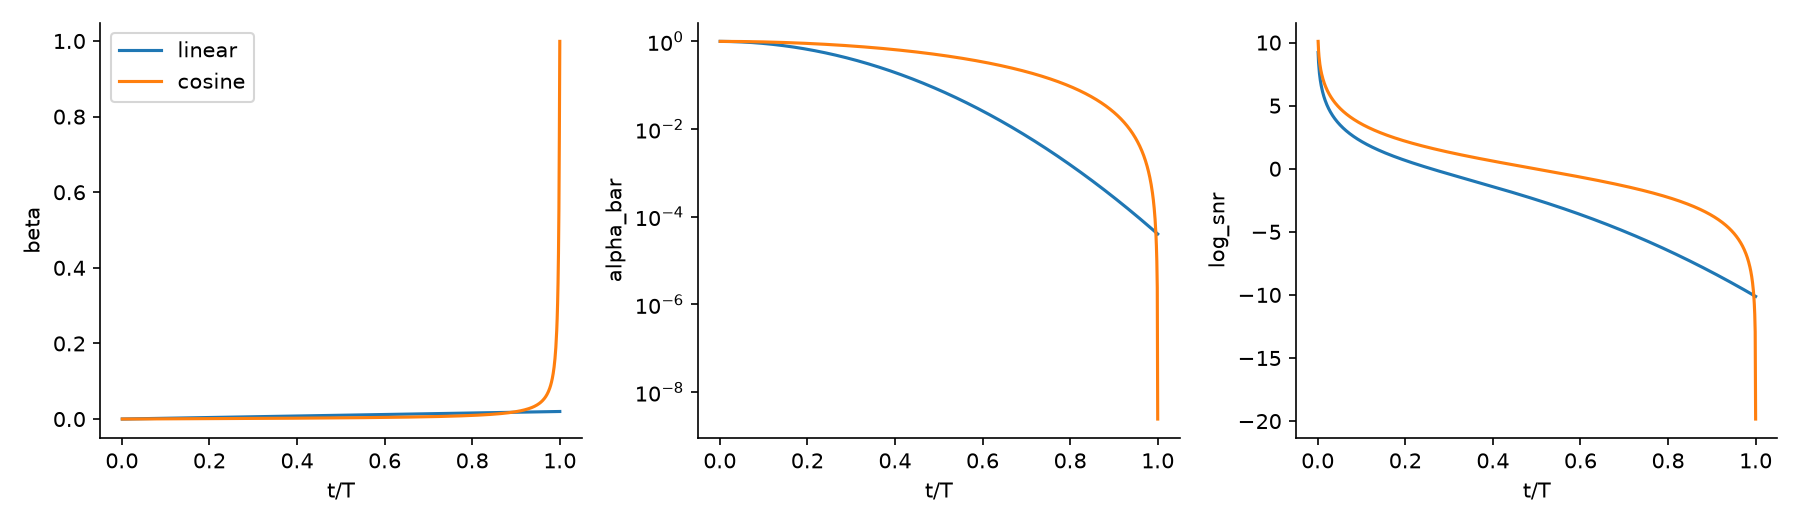
\includegraphics[width=\linewidth,height=.37\textheight,keepaspectratio]{figures/schedules.png}
\caption{E1: beta, накопленный сигнал и log SNR двух расписаний.}\label{fig:schedules}
\end{figure}

Для фиксированного $x_0$ получено 10 000 независимых шумовых реализаций на каждом из пяти t. Все координаты прошли исходную проверку четырёх стандартных ошибок; seed не подбирался (R29).
\begin{table}[H]\centering\footnotesize
\setlength{\tabcolsep}{4pt}
\caption{Проверка q sample: максимальная по координатам ошибка среднего и относительная ошибка дисперсии.}\label{tab:moments}
\begin{tabular}{llrrrr}
\toprule
Schedule & $t$ & $\max|\hat m-m|$ & Порог & $\max|\hat v/v-1|$ & Порог \\
\midrule
linear & 100 & 0.004218 & 0.012836 & 0.010893 & 0.056569 \\
linear & 250 & 0.007435 & 0.027595 & 0.009194 & 0.056569 \\
linear & 500 & 0.010862 & 0.038396 & 0.008333 & 0.056569 \\
linear & 750 & 0.007942 & 0.039933 & 0.017253 & 0.056569 \\
linear & 1000 & 0.008787 & 0.039999 & 0.030062 & 0.056569 \\
cosine & 100 & 0.002196 & 0.006682 & 0.010893 & 0.056569 \\
cosine & 250 & 0.004215 & 0.015645 & 0.009194 & 0.056569 \\
cosine & 500 & 0.008051 & 0.028458 & 0.008333 & 0.056569 \\
cosine & 750 & 0.007359 & 0.037002 & 0.017253 & 0.056569 \\
cosine & 1000 & 0.008788 & 0.040000 & 0.030062 & 0.056569 \\
\bottomrule
\end{tabular}
\end{table}


\begin{figure}[H]\centering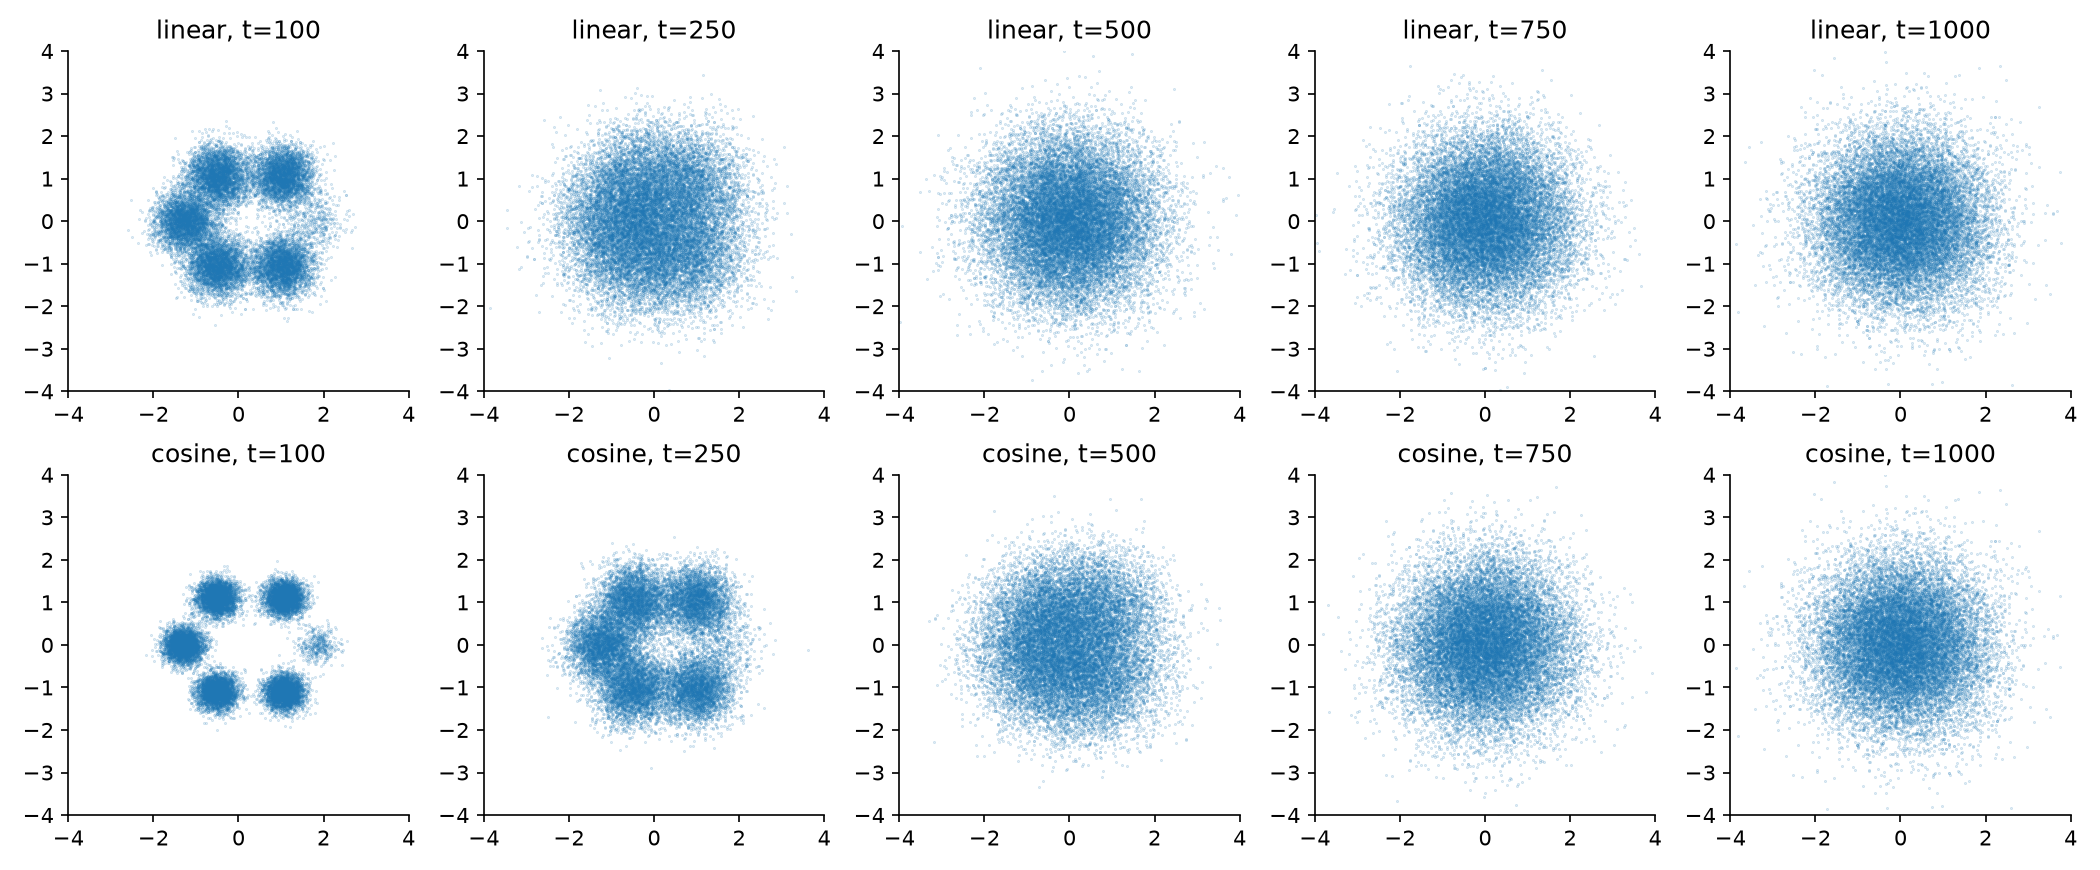
\includegraphics[width=\linewidth,height=.35\textheight,keepaspectratio]{figures/clouds.png}
\caption{Прямой процесс при пяти уровнях шума.}\label{fig:clouds}
\end{figure}

\begin{figure}[H]\centering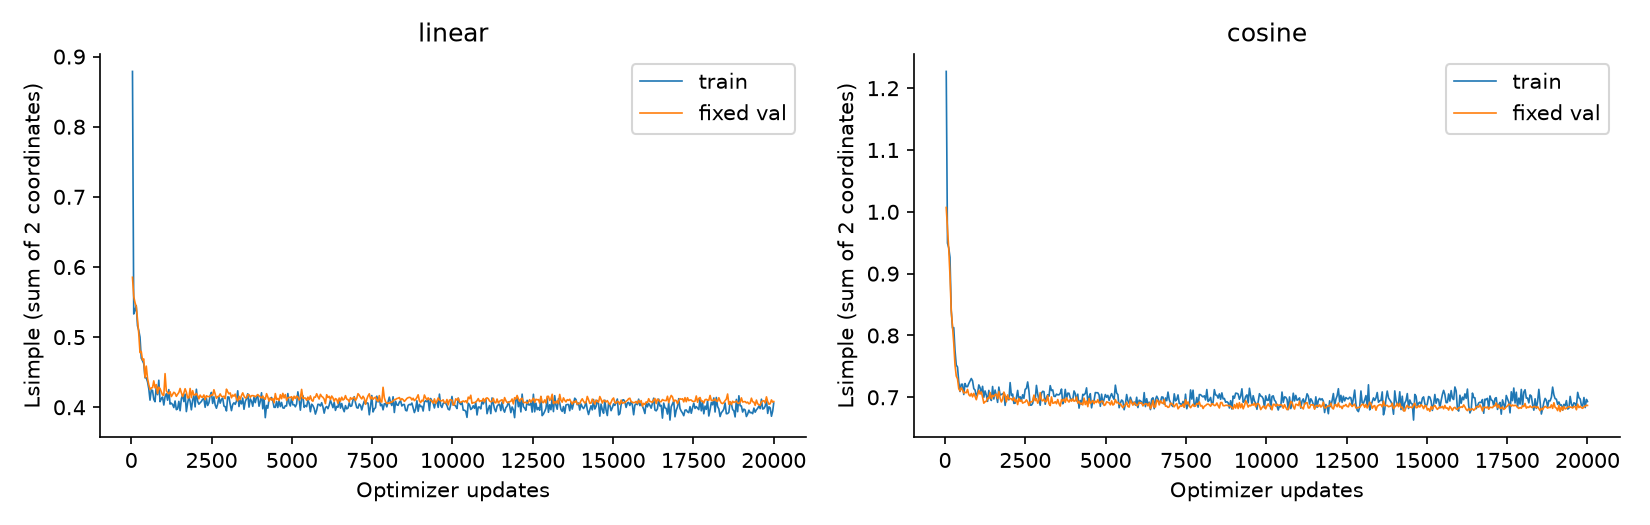
\includegraphics[width=\linewidth,height=.35\textheight,keepaspectratio]{figures/training.png}
\caption{E1: train и фиксированный val loss при 20 000 обновлений.}\label{fig:training}
\end{figure}

\begin{figure}[H]\centering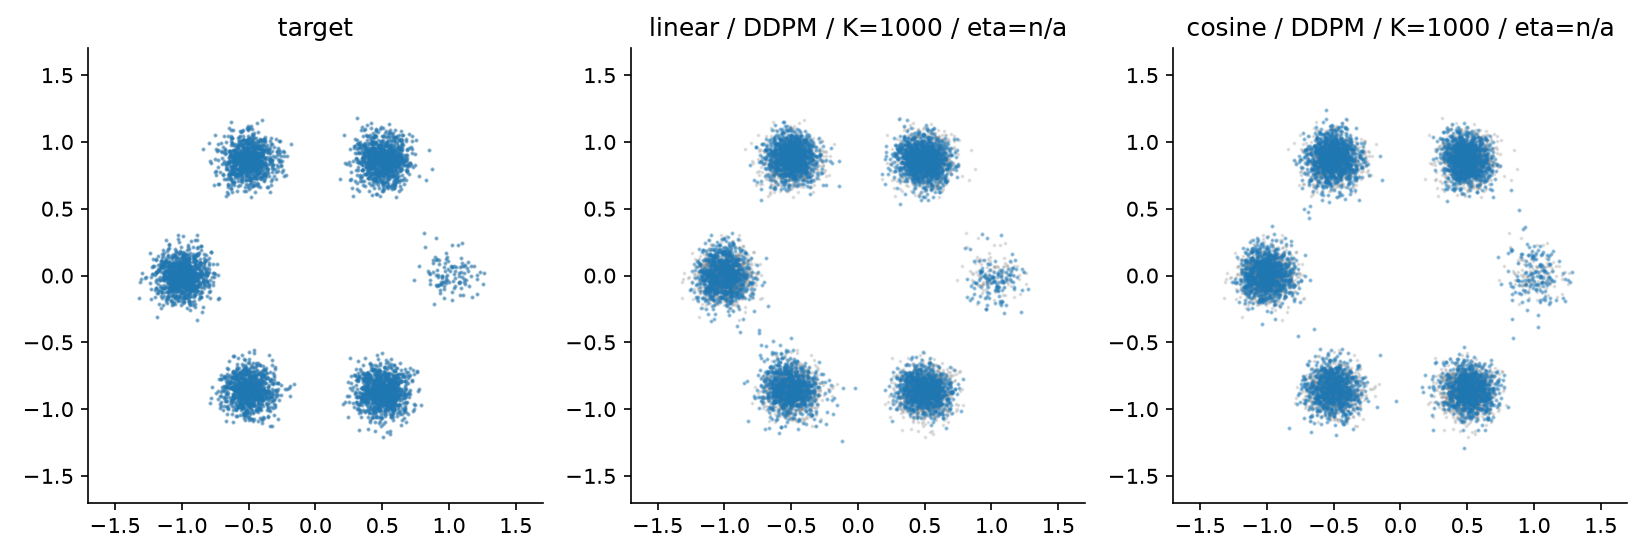
\includegraphics[width=\linewidth,height=.36\textheight,keepaspectratio]{figures/samples.png}
\caption{E1: linear и cosine, DDPM K=1000, posterior variance, без clipping.}\label{fig:samples}
\end{figure}

Граница применимости: $T=100$ при прежних beta даёт $\bar\alpha_T=0.363563$, KL=0.451870, нарушая конечный порог. Это отдельная диагностика точного предиктора, не формальное обучение. Exact DDPM дал MMD$^2=0.000072387$, Dmode=0.01229 (R30), против 0.000139853 и 0.01627 при полном T. В одном измерении ухудшения нет. Условный KL из формулы не равен KL смеси к нормальному шуму, поэтому наблюдение не отменяет протокольный порог и не доказывает пользу его нарушения.

\section{E2. Качество и стоимость сэмплирования}
Linear-модель E1 заморожена. Меняется только обратная схема; начальные шумы общие, для стохастических шагов зафиксирован отдельный seed. Сеть не переобучается при смене K. Exact --- отдельный предиктор, не обученная сеть.
\begin{table}[H]\centering\footnotesize
\setlength{\tabcolsep}{4pt}
\caption{E2: общий начальный шум; время --- медиана пяти повторов после прогрева.}\label{tab:sampling}
\begin{tabular}{llrrrrrl}
\toprule
Предиктор & Сэмплер & NFE & MMD$^2$ & $D_{mode}$ & Cov & Время, с & Ист. \\
\midrule
network & ddpm & 1000 & 0.0021705 & 0.05625 & 1.000 & 1.61582 & R03 \\
network & ddim & 5 & 0.0516226 & 0.66303 & 0.167 & 0.00899 & R04 \\
network & ddim & 10 & 0.0147229 & 0.21945 & 1.000 & 0.01749 & R05 \\
network & ddim & 20 & 0.0085653 & 0.12585 & 1.000 & 0.04071 & R06 \\
network & ddim & 50 & 0.0066821 & 0.09245 & 1.000 & 0.08617 & R07 \\
network & ddim & 100 & 0.0060813 & 0.08865 & 1.000 & 0.17946 & R08 \\
network & ddim & 1000 & 0.0056764 & 0.08525 & 1.000 & 1.82389 & R09 \\
exact & ddpm & 1000 & 0.0001399 & 0.01627 & 1.000 & 2.05166 & R10 \\
exact & ddim & 5 & 0.0140085 & 0.48883 & 0.500 & 0.01182 & R11 \\
exact & ddim & 10 & 0.0010714 & 0.12103 & 1.000 & 0.02350 & R12 \\
exact & ddim & 20 & 0.0002459 & 0.01882 & 1.000 & 0.04725 & R13 \\
exact & ddim & 50 & 0.0000802 & 0.01152 & 1.000 & 0.11504 & R14 \\
exact & ddim & 100 & 0.0000507 & 0.01292 & 1.000 & 0.24209 & R15 \\
exact & ddim & 1000 & 0.0000395 & 0.01169 & 1.000 & 2.37442 & R16 \\
\bottomrule
\end{tabular}
\end{table}


\begin{figure}[H]\centering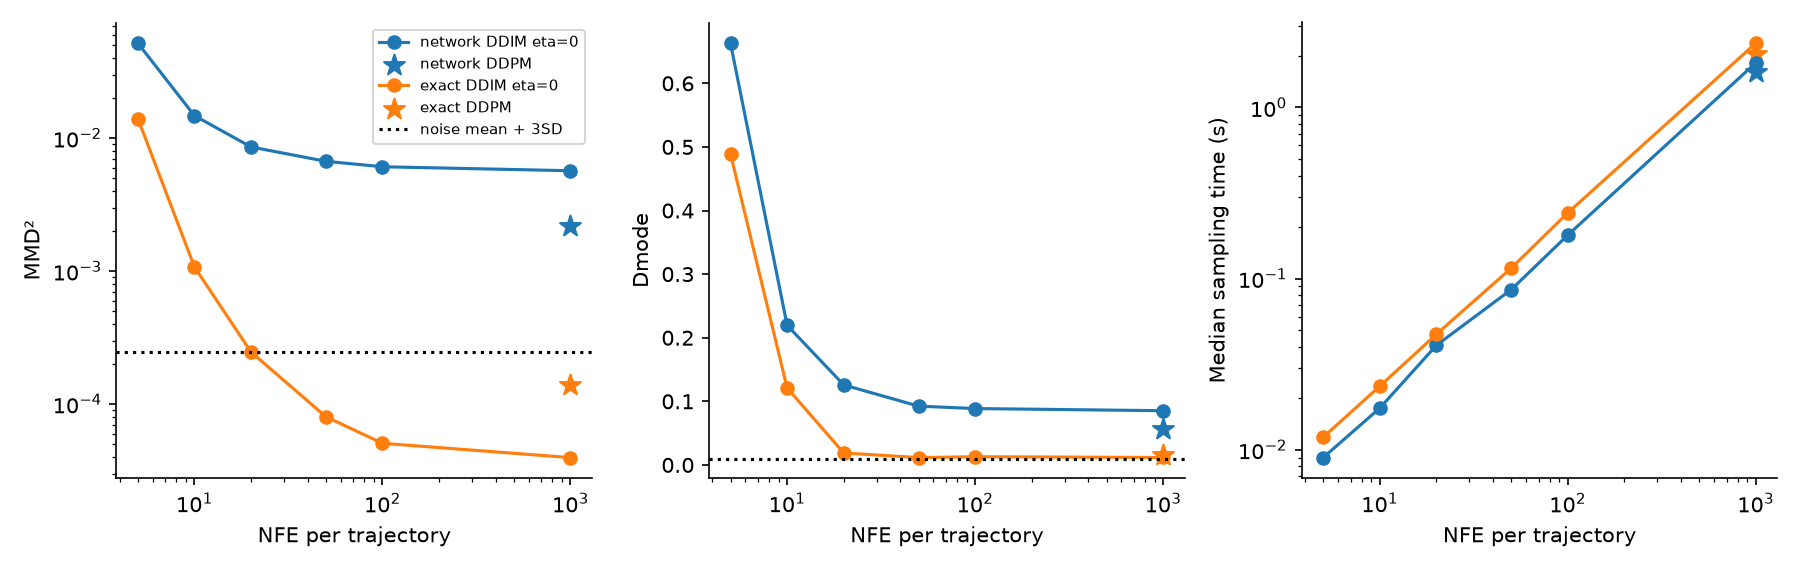
\includegraphics[width=\linewidth,height=.43\textheight,keepaspectratio]{figures/cost.png}
\caption{E2: качество и время от NFE, linear; DDIM eta=0, DDPM posterior variance.}\label{fig:cost}
\end{figure}

NFE на траекторию равен T у DDPM и K у DDIM. Для $K\ge10$ времена на вызов укладываются в 20\% от соответствующей медианы: максимум отклонения сети 16.37\%, точного предиктора 12.68\%. При полном T точный DDPM и DDIM ниже порога MMD$^2=0.000245055$ (шум плюс три SD). Рост ошибки exact при малых K показывает вклад численной схемы, разрыв network--exact при том же K --- вклад сети.

Для DDIM T использованы три начальных шума. Значения MMD$^2$: 0.005676381, 0.006164185 и 0.004929829; $s_{MMD}=0.000621681$. Критерий
\begin{equation}|MMD^2(K)-MMD^2(T)|\le2s_{MMD}=0.001243363\end{equation}
впервые выполняется на измеренной сетке при $K=50$. Это минимум сетки, а не точный оптимум среди всех целых K.
\begin{table}[H]\centering\small
\setlength{\tabcolsep}{4pt}
\caption{Крайне малое число шагов DDIM; отдельная оценка, без заявления о пяти повторах времени.}\label{tab:low}
\begin{tabular}{llrrrl}
\toprule
Предиктор & K & MMD$^2$ & $D_{mode}$ & Cov & Ист. \\
\midrule
network & 1 & 0.573304 & 0.98063 & 0.000 & R17 \\
network & 2 & 0.128446 & 0.98563 & 0.000 & R18 \\
exact & 1 & 0.130350 & 0.98903 & 0.000 & R19 \\
exact & 2 & 0.107975 & 0.98863 & 0.000 & R20 \\
\bottomrule
\end{tabular}
\end{table}


\begin{figure}[H]\centering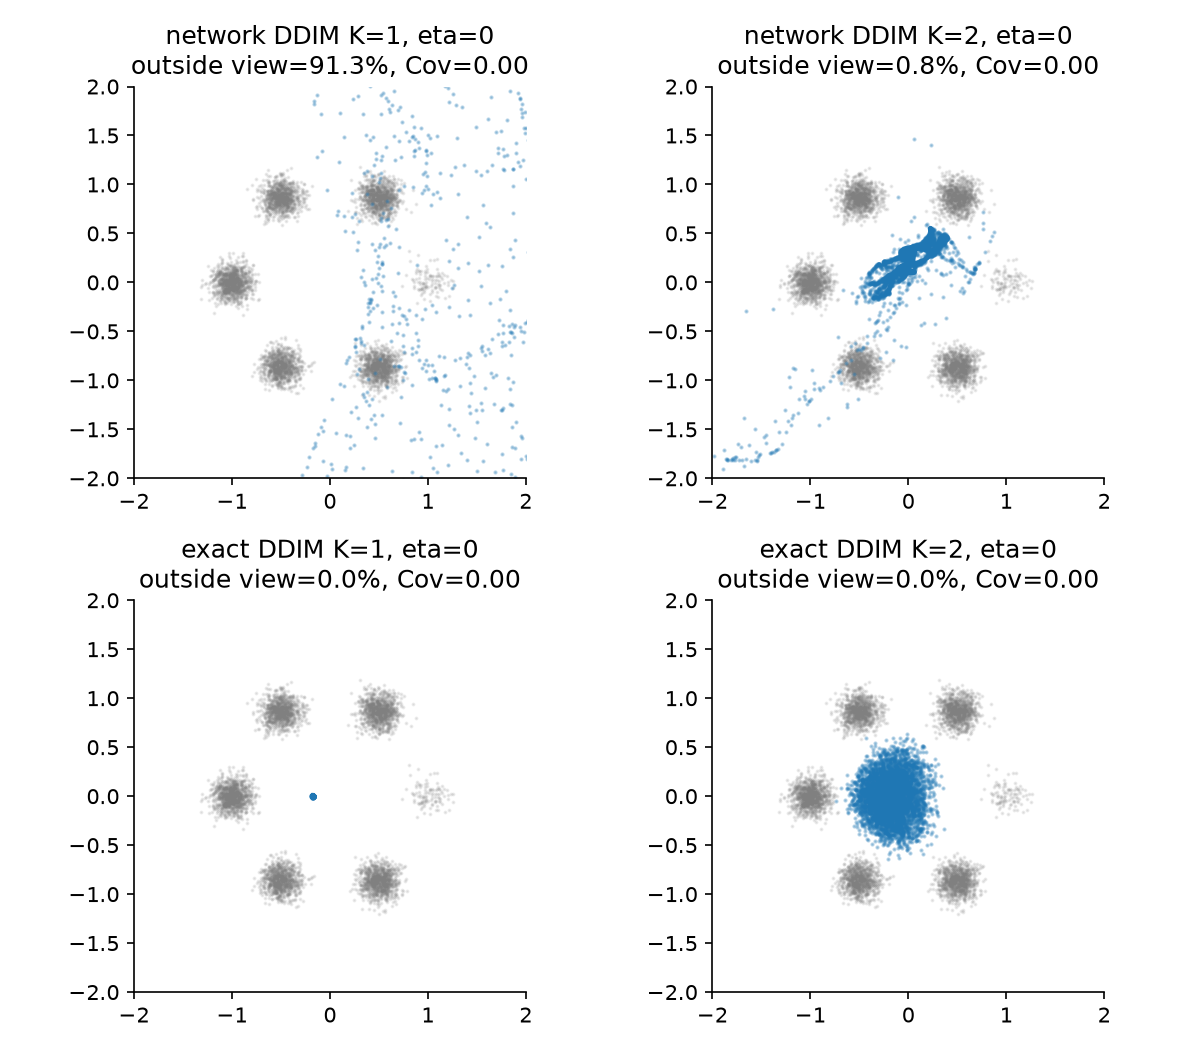
\includegraphics[width=\linewidth,height=.38\textheight,keepaspectratio]{figures/extreme.png}
\caption{Linear DDIM eta=0, K=1 и 2: сеть и точный предиктор.}\label{fig:extreme}
\end{figure}

При K=1 точный DDIM возвращает Tweedie posterior mean, лежащий между модами при почти чистом шуме; Cov=0. При K=2 покрытие также нулевое, а при K=5 появляются покрытые моды: exact Cov=0.5, сеть 0.1667. С K=10 оба предиктора достигают Cov=1, хотя частоты и MMD ещё различаются.

\section{Диагностика сети и траекторий}
Ошибки рассчитаны на общих фиксированных val и шуме в 25 t, включая 1 и T:
\begin{equation}E_\epsilon=\tfrac1dE\|\epsilon-\epsilon_\theta\|^2,\quad E_{x_0}=E_\epsilon/SNR,\quad E_{net}=\tfrac1dE\|\epsilon_*-\epsilon_\theta\|^2.\end{equation}
В ожидании $E_\epsilon=E^*_\epsilon+E_{net}$. На конечной выборке сохраняется измеренный перекрёстный член с SEM; его не обнуляют принудительно. Для exact собственная ошибка равна нулю.
\begin{figure}[H]\centering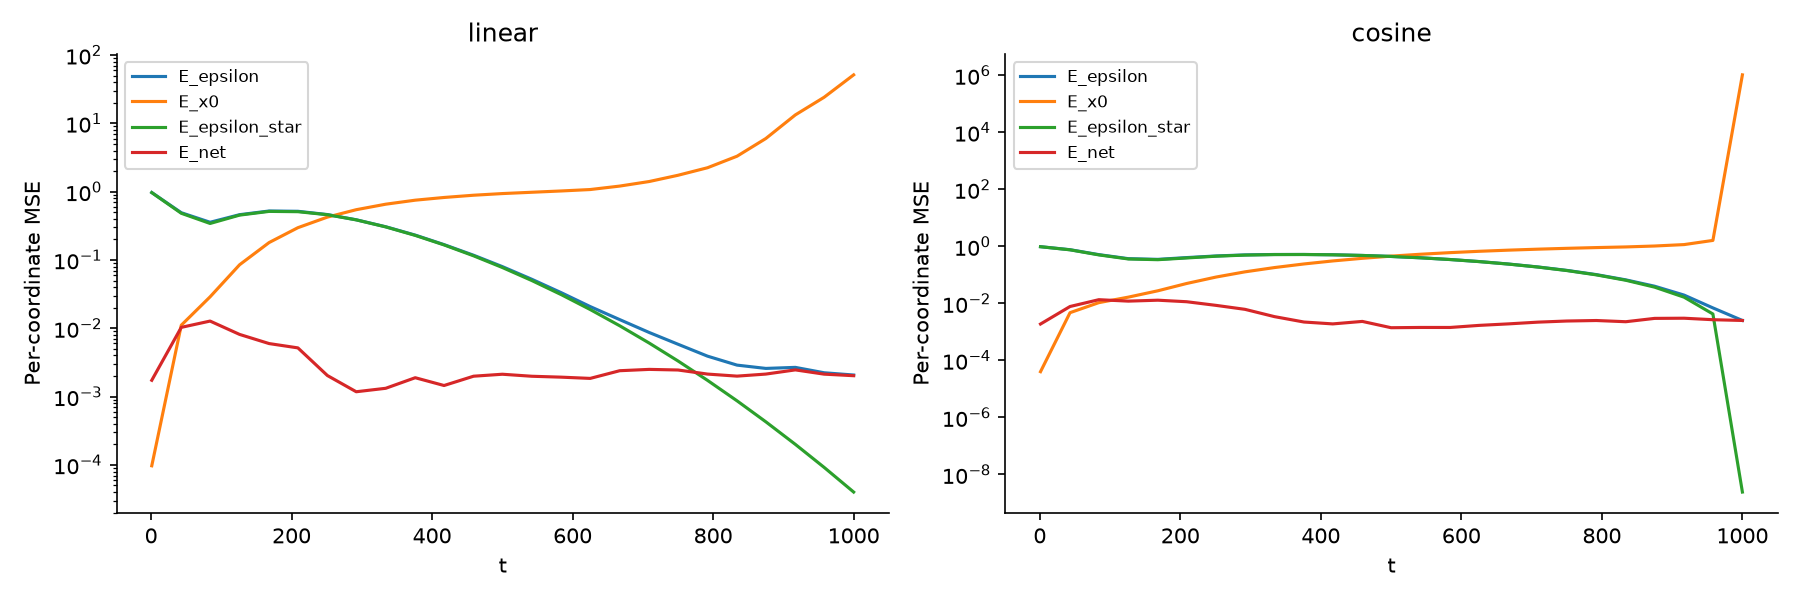
\includegraphics[width=\linewidth,height=.41\textheight,keepaspectratio]{figures/timestep.png}
\caption{Ошибки на 25 шагах для двух расписаний, фиксированные val и шум.}\label{fig:timestep}
\end{figure}

На T linear имеет $E_\epsilon=0.002069320$, $E^*_\epsilon=0.000040065$, $E_{net}=0.002022949$, $E_{x_0}=51.271643$. Cosine: 0.002514774, $2.4111\cdot10^{-9}$, 0.002514743 и $1.035412\cdot10^6$. Разные единицы ошибок принципиальны: маленькая ошибка epsilon при низком SNR может дать большую ошибку восстановления.
\begin{table}[H]\centering\small
\setlength{\tabcolsep}{4pt}
\caption{Score на сетке $41\times41$: средние с весами $p_t(x)$.}\label{tab:fields}
\begin{tabular}{llrrl}
\toprule
Schedule & $t$ & Косинус & Отношение длин & Ист. \\
\midrule
linear & 10 & 0.979138 & 1.099804 & R21 \\
linear & 100 & 0.967361 & 0.978513 & R21 \\
linear & 400 & 0.996687 & 1.028544 & R21 \\
linear & 800 & 0.995145 & 1.602079 & R21 \\
cosine & 10 & 0.974234 & 1.214775 & R22 \\
cosine & 100 & 0.986461 & 0.964783 & R22 \\
cosine & 400 & 0.985098 & 1.027589 & R22 \\
cosine & 800 & 0.987465 & 1.067802 & R22 \\
\bottomrule
\end{tabular}
\end{table}


\begin{figure}[H]\centering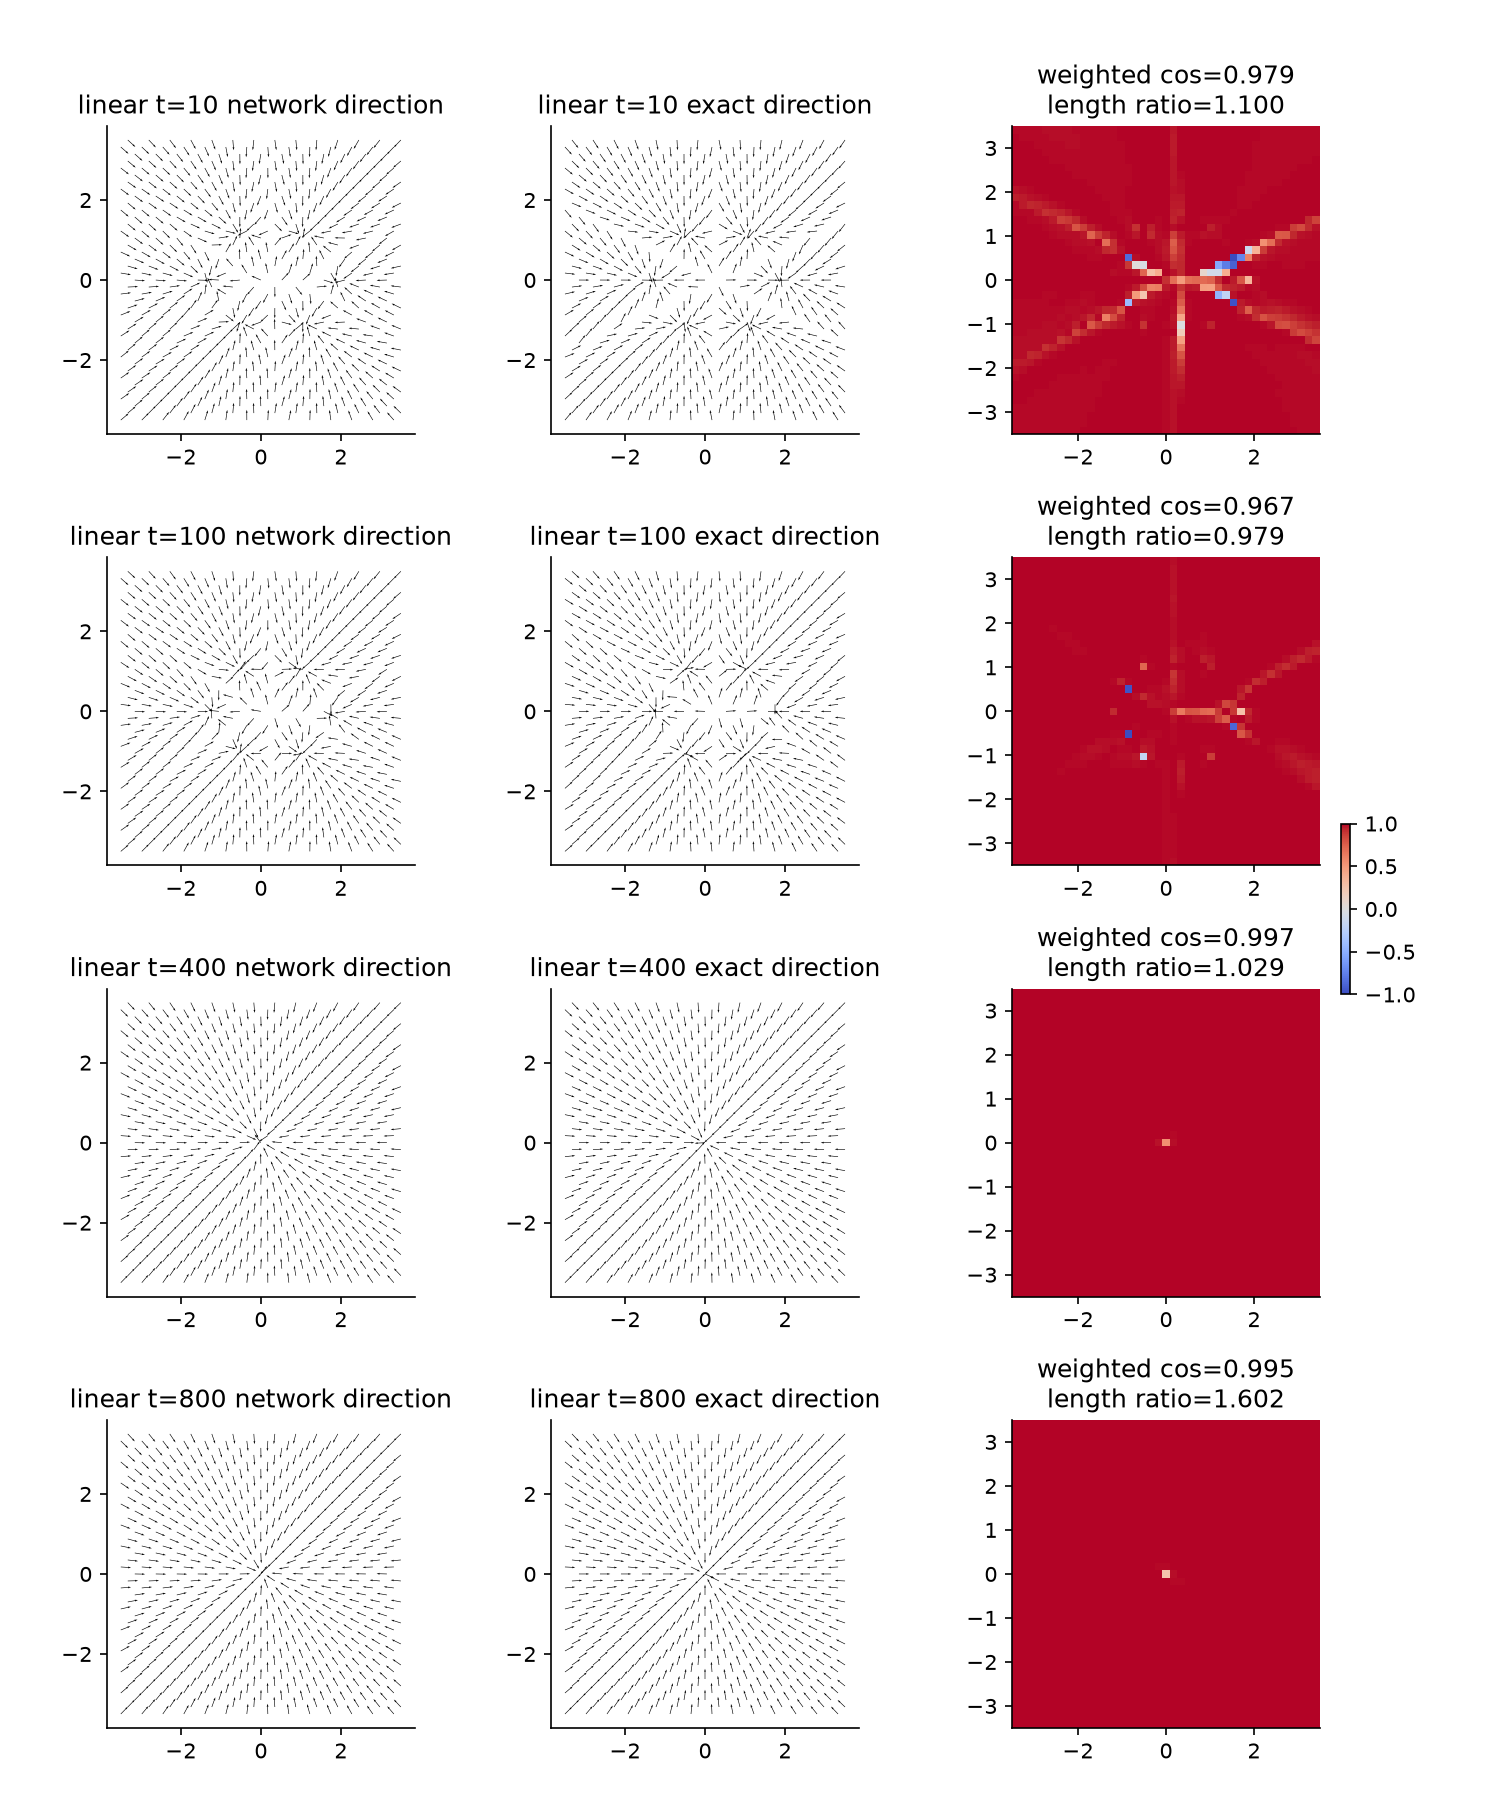
\includegraphics[width=\linewidth,height=.53\textheight,keepaspectratio]{figures/scorelinear.png}
\caption{Linear: поля score, косинусы и длины на четырёх уровнях шума.}\label{fig:scorelinear}
\end{figure}

\begin{figure}[H]\centering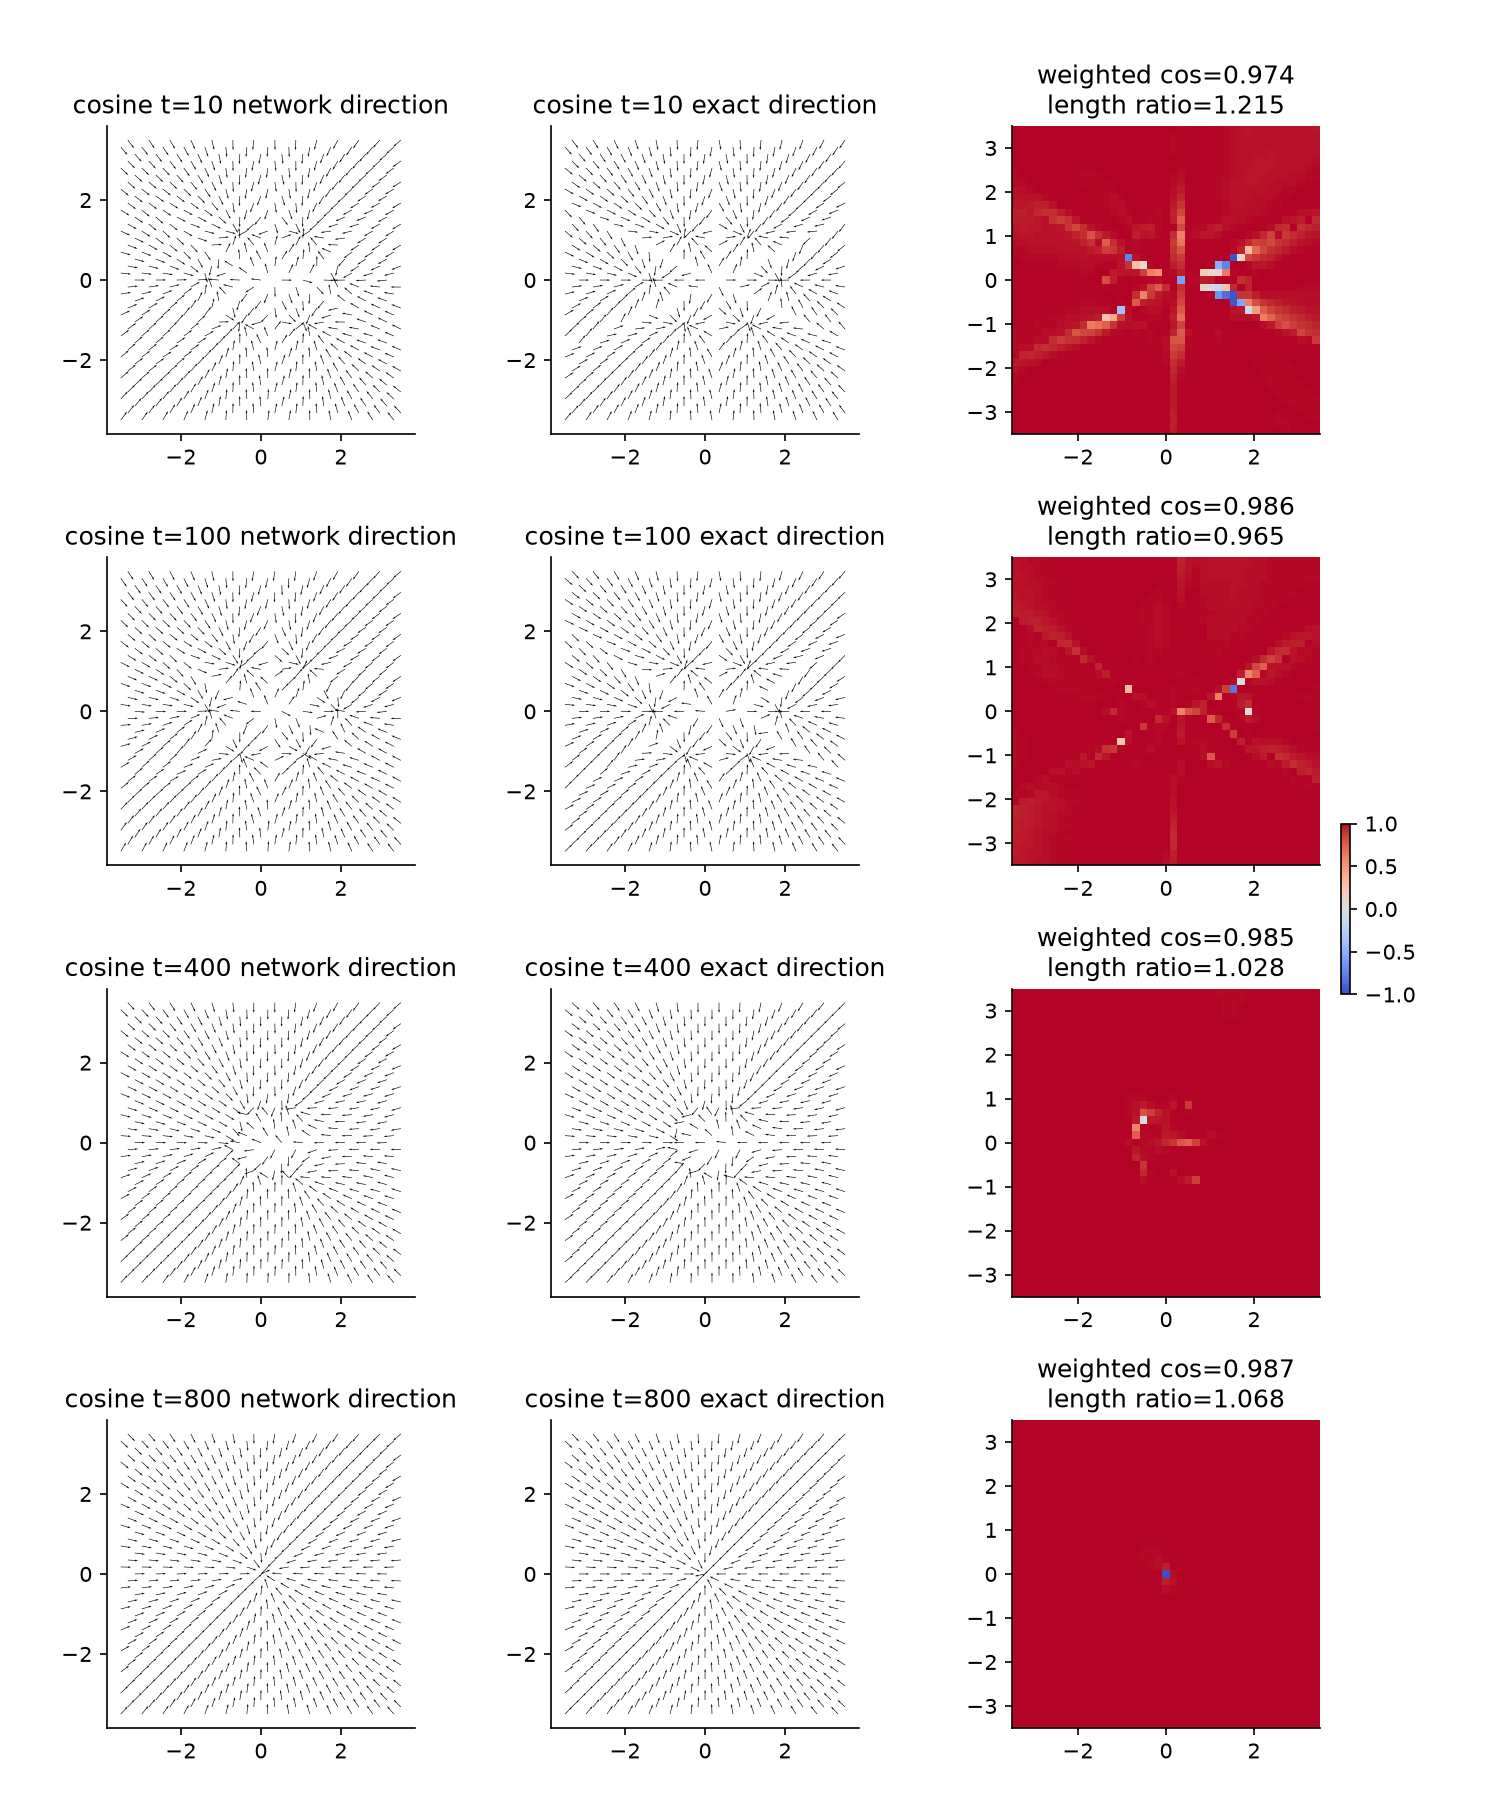
\includegraphics[width=\linewidth,height=.53\textheight,keepaspectratio]{figures/scorecosine.png}
\caption{Cosine: аналогичная диагностика с весами вероятностной массы.}\label{fig:scorecosine}
\end{figure}

Косинусы высоки, но отношение длин не всегда близко к 1: например linear t=800 даёт 1.602079. Вероятностные веса $p_t$ предотвращают преобладание пустых областей над выводом о поле.
\begin{table}[H]\centering\small
\setlength{\tabcolsep}{4pt}
\caption{Доля 1000 траекторий DDPM, направленных к итоговой моде.}\label{tab:trajectory}
\begin{tabular}{rrr}
\toprule
$t/T$ & Linear & Cosine \\
\midrule
0.8 & 0.155 & 0.285 \\
0.6 & 0.197 & 0.416 \\
0.4 & 0.336 & 0.667 \\
0.2 & 0.67 & 0.943 \\
0.05 & 0.989 & 0.991 \\
\bottomrule
\end{tabular}
\end{table}


\begin{figure}[H]\centering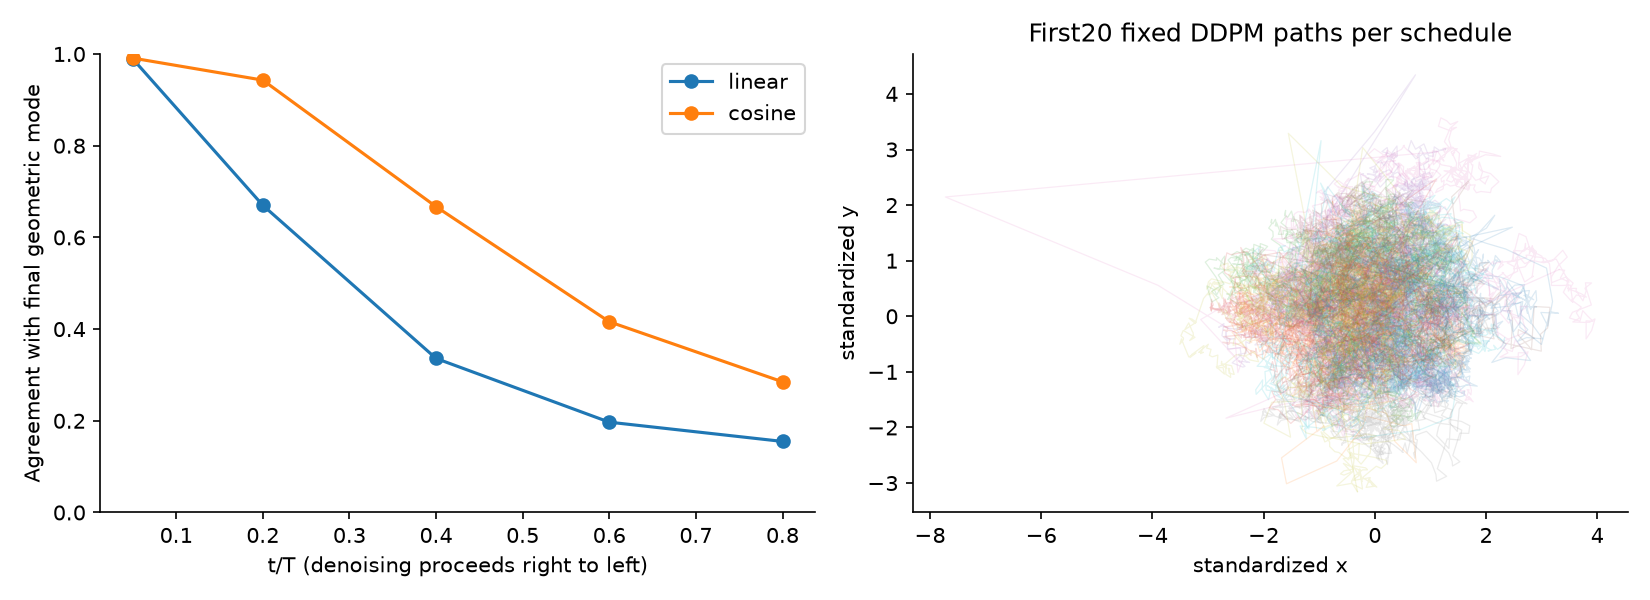
\includegraphics[width=\linewidth,height=.35\textheight,keepaspectratio]{figures/traj.png}
\caption{1000 DDPM-траекторий и постепенное формирование моды.}\label{fig:traj}
\end{figure}

Начальные шумы фиксированы, для каждой модели сохранено 1000 полных DDPM-траекторий (R31 / R32). Ближайший масштабированный центр сравнивается с финальной модой. У linear выбор формируется позднее по индексу t, чем у cosine; индексы соответствуют разным SNR. Рост согласия постепенный, единственный универсальный момент выбора не установлен.

\section{E3. Покрытие редкой моды}
A --- linear DDPM, T=1000, posterior variance; B --- DDIM K=50, eta=0 на тех же весах. Единственный фактор --- конфигурация обратного сэмплера. Фиксированы данные, стандартизация, архитектура, полоса, обучение и общий $x_T$. До дополнительных seed предсказан отрицательный знак $Dmode(A)-Dmode(B)$ из-за дискретизационной ошибки малого K; отсутствие устойчивого отрицательного различия опровергло бы прогноз. Seed 1 явно повторно использует E1/E2, seed 2 и 3 проведены после фиксации гипотезы.
\begin{table}[H]\centering\small
\setlength{\tabcolsep}{4pt}
\caption{E3: A --- DDPM T, B --- DDIM 50; общая linear-сеть внутри seed.}\label{tab:e3}
\begin{tabular}{llrrrrl}
\toprule
Seed & Arm & Cov & $\hat p_0$ & $D_{mode}$ & MMD$^2$ & Ист. \\
\midrule
1 & A & 1.0 & 0.0238 & 0.05625 & 0.00217049 & R03 \\
1 & B & 1.0 & 0.0320 & 0.09245 & 0.00668209 & R07 \\
2 & A & 1.0 & 0.0176 & 0.02143 & 0.00049002 & R23 \\
2 & B & 1.0 & 0.0146 & 0.06917 & 0.00150298 & R24 \\
3 & A & 1.0 & 0.0300 & 0.02502 & 0.00040347 & R25 \\
3 & B & 1.0 & 0.0308 & 0.07214 & 0.00142802 & R26 \\
\bottomrule
\end{tabular}
\end{table}


\begin{figure}[H]\centering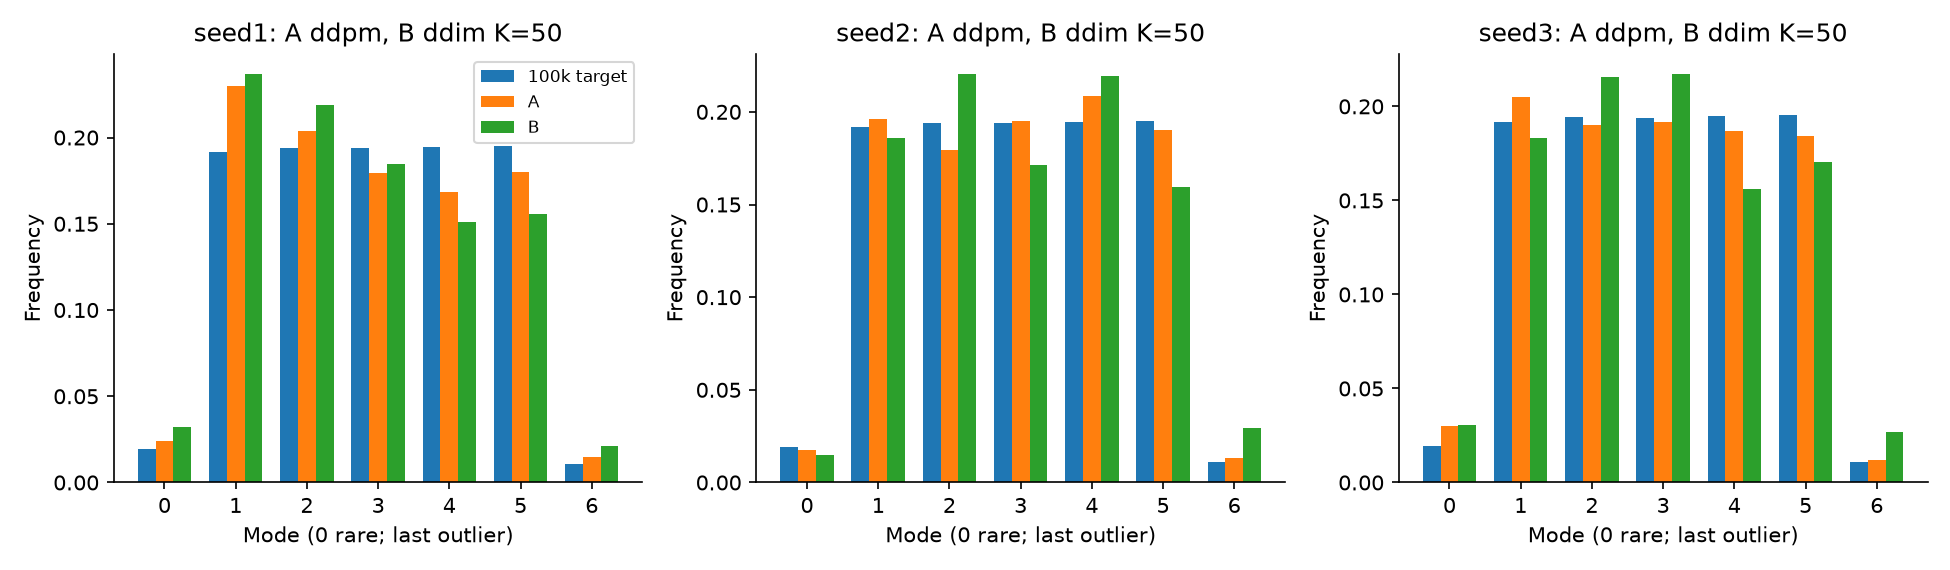
\includegraphics[width=\linewidth,height=.42\textheight,keepaspectratio]{figures/modes.png}
\caption{E3: полные частоты шести мод и внешней категории; linear, DDPM T / DDIM 50 eta=0.}\label{fig:modes}
\end{figure}

\begin{figure}[H]\centering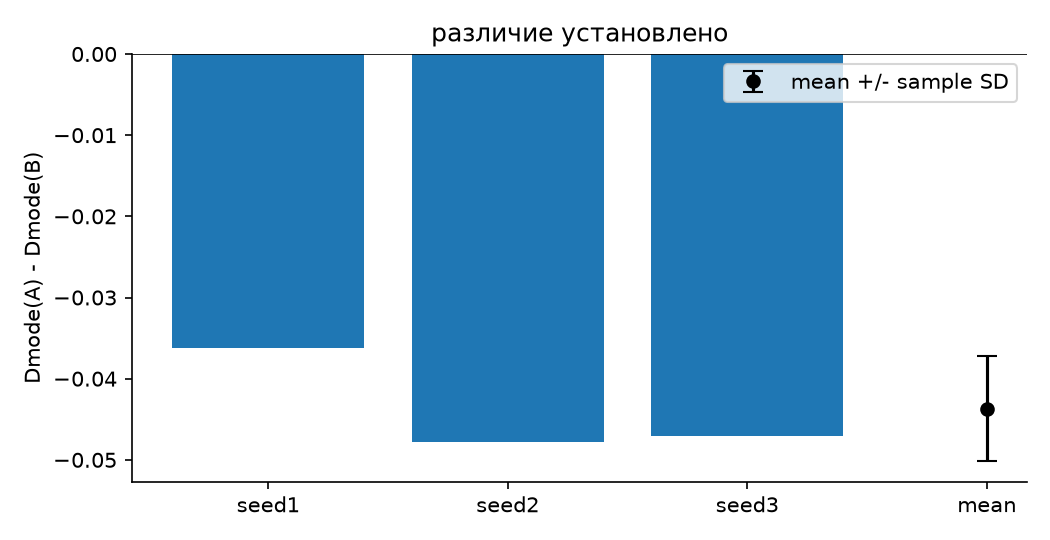
\includegraphics[width=\linewidth,height=.28\textheight,keepaspectratio]{figures/pairs.png}
\caption{Три парные разности Dmode: DDPM минус DDIM 50.}\label{fig:pairs}
\end{figure}

Три разности $-0.03620,-0.04774,-0.04712$, среднее $-0.043686667$, выборочное SD 0.006491050. Знаки одинаковы, модуль среднего выше $2s_\Delta=0.012982101$ и шума Dmode=0.009434: различие установлено в пользу A, гипотеза поддержана. Все редкие частоты превышают $\pi_0/2=0.01$. Смена seed не переносит вывод на другие цели.
\begin{table}[H]\centering\small
\setlength{\tabcolsep}{4pt}
\caption{Новый target и полное обучение A при уменьшенном весе редкой моды.}\label{tab:rare}
\begin{tabular}{rrrrrl}
\toprule
$\pi_0$ & Train: компонент 0 & $\hat p_0$ & Cov & $D_{mode}$ & Ист. \\
\midrule
0.01 & 199 & 0.0102 & 1.0 & 0.05335 & R27 \\
0.005 & 113 & 0.0050 & 1.0 & 0.05564 & R28 \\
\bottomrule
\end{tabular}
\end{table}


\begin{figure}[H]\centering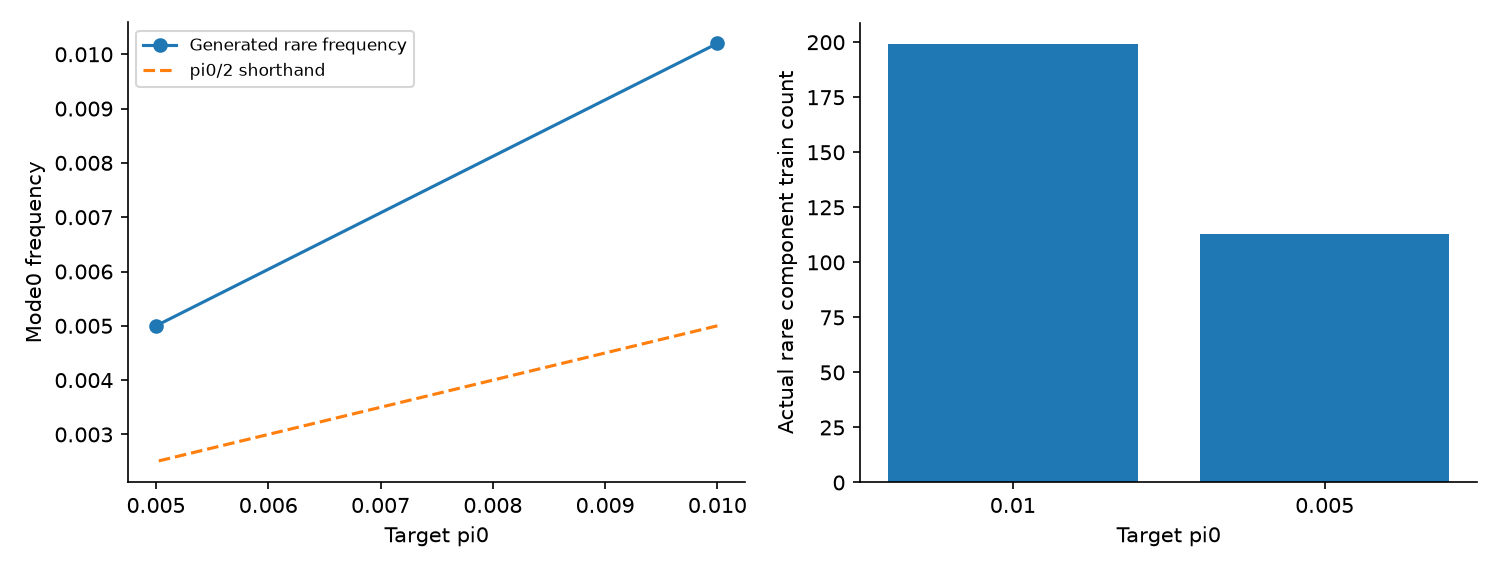
\includegraphics[width=\linewidth,height=.32\textheight,keepaspectratio]{figures/rarefig.png}
\caption{Дополнительные A-модели с pi0/2 и pi0/4; linear DDPM T.}\label{fig:rarefig}
\end{figure}

Для каждого меньшего веса созданы новые train/val/test, заново рассчитаны train-статистики и обучена отдельная A-модель полные 20 000 шагов. При $\pi_0=0.01$ и 0.005 редкая мода остаётся покрытой: $\hat p_0=0.0102$ и 0.0050. Точка потери покрытия в проверенном диапазоне не найдена; неизвестный порог не экстраполируется.

\section{Ответы на контрфактические вопросы}
\subsection*{Вопрос 1. Десятикратное T}
Сохранённое дополнительное обучение при T=10 000 и прежних beta содержит 20 000 обновлений (R33). $\bar\alpha_T=1.146727\cdot10^{-44}$, средний условный KL такой же по порядку, против $4.035911\cdot10^{-5}$ при T=1000. NFE вырос в 10 раз, медианное время DDPM --- в 11.702753 раза. MMD$^2$ снизилась с 0.002170494 до 0.000369903, Dmode с 0.05625 до 0.02903, Cov=1. Улучшение наблюдалось в одном seed; оно не является необходимым следствием меньшего конечного KL, поскольку меняется и распределение обучающих задач по времени.
\subsection*{Вопрос 2. Нулевой предиктор}
Для $\epsilon_\theta=0$ имеем $v_T=1$, $v_{t-1}=v_t/\alpha_t+\tilde\beta_t$ при $t>1$, $v_0=v_1/\alpha_1$ без последнего шума. Расчёт даёт 49 085.039063, реальные 5000 точек --- дисперсии 49 473.790459 и 49 843.273129, ошибки 0.792\% и 1.545\% (R34). Без оценки шума обратная цепь расширяет облако и не направляет его к данным.
\begin{figure}[H]\centering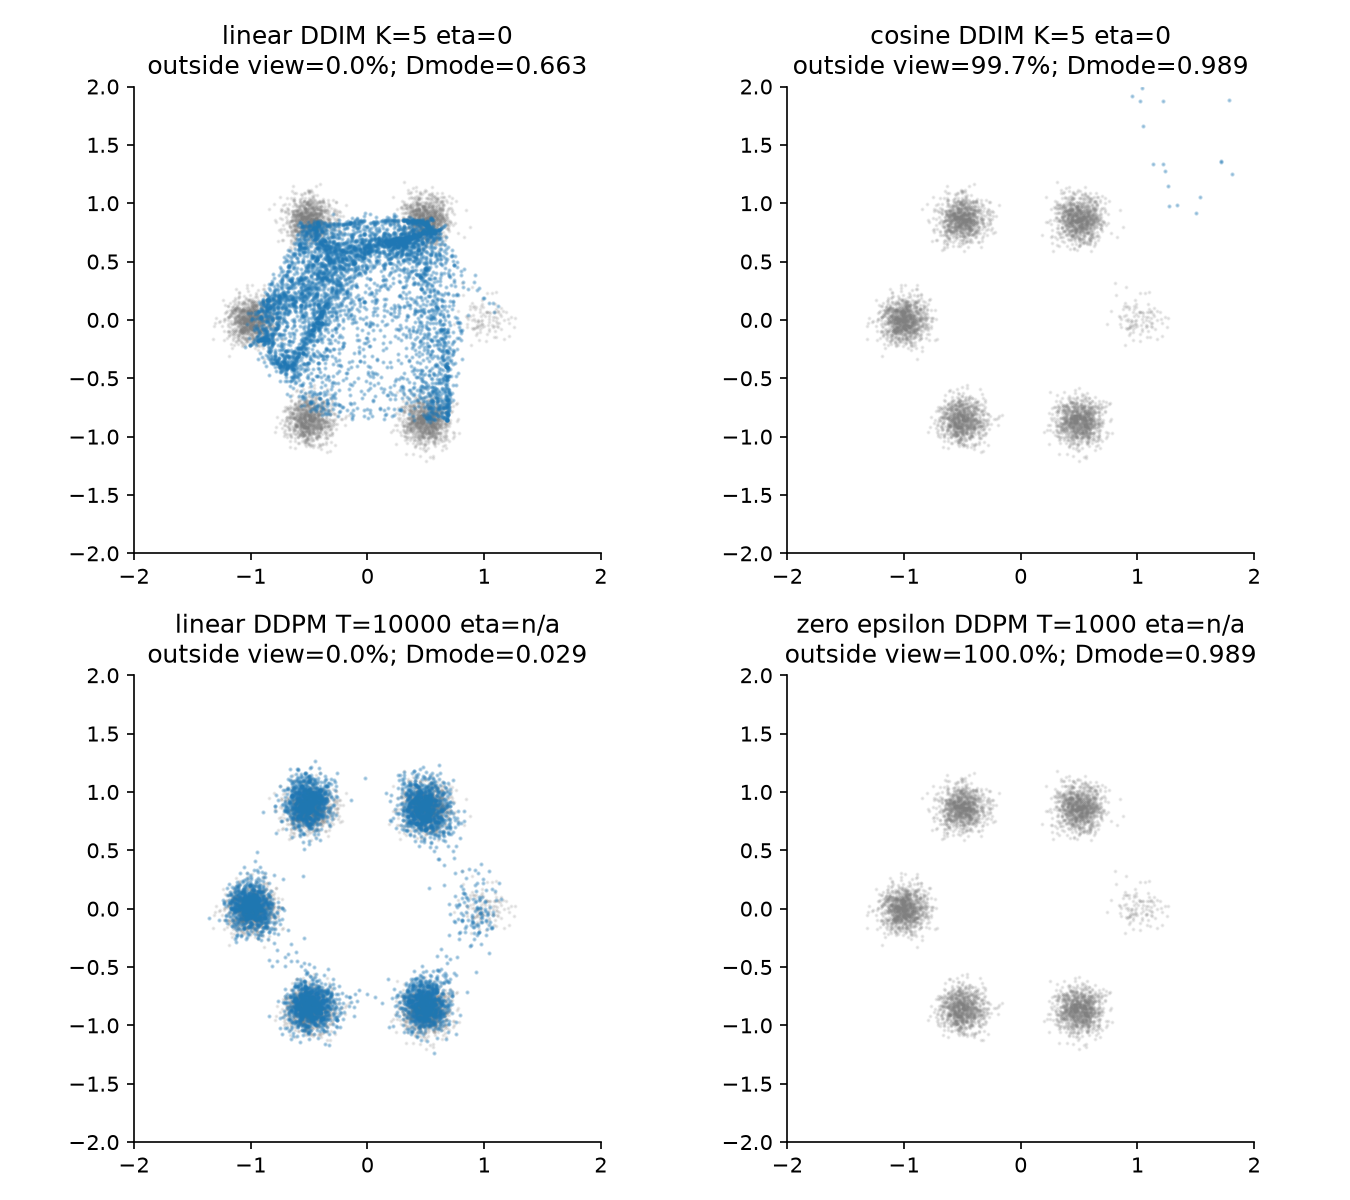
\includegraphics[width=\linewidth,height=.30\textheight,keepaspectratio]{figures/controls.png}
\caption{Контрфактические оценки: короткое T, десятикратное T и нулевой предиктор.}\label{fig:controls}
\end{figure}

\subsection*{Вопрос 3. Loss и качество}
Linear/cosine val loss 0.408203/0.686859, MMD$^2$ 0.002170494/0.002191699, Dmode 0.05625/0.05185. Linear лучше по численной MMD, cosine по Dmode; различия малы относительно шума. Равномерные t в разных расписаниях дают разные смеси задач: linear имеет 32.6\% низкого SNR, cosine 6.4\%. Высокий шум облегчает epsilon prediction, но не восстановление x0. Поэтому $L_{simple}$ не заменяет качество и не является точным NLL.
\subsection*{Вопрос 4. Усиление терминальной ошибки}
$E_{net}(T)/SNR(T)$ равно 50.122722 для linear и 1 035 399.171539 для cosine. Это MSE относительно точного posterior mean на первом шаге, а не финальная MMD. При DDIM K=5 linear даёт Cov=0.1667, MMD$^2=0.051623$, cosine Cov=0, MMD$^2=0.600008$ (R35). Данные согласуются с сильным усилением ошибки малого SNR; последующие шаги способны частично её исправить, поэтому прямого равенства с финальным качеством нет.
\subsection*{Вопрос 5. Cov недостаточно}
Среди формальных E3 с Cov=1 максимальный Dmode=0.09245 у seed 1, B. Частоты мод 0--5 и внешней категории: 0.0320,0.2366,0.2188,0.1844,0.1512,0.1558,0.0212. Мода 4 недооценена на 0.04349, мода 1 переоценена на 0.04490; редкая мода имеет 0.0320 против справочных 0.01931. Дополнительные траектории этой DDIM-конфигурации дают согласия с финальной модой 0.696,0.712,0.783,0.880,0.981 при t=800,600,400,200,60 (для запроса 50 использован ближайший сохранённый tau=60). Cov допускает дисбаланс и внешние точки; нужны полные частоты и Dmode.

\noindent\textbf{Заключение.} DDPM точнее по частотам, DDIM 50 быстрее.
\clearpage
\renewcommand{\refname}{Список использованных источников}
\begin{thebibliography}{9}
\addcontentsline{toc}{section}{Список использованных источников}
\bibitem{teacher} Лабораторная работа 7. Diffusion и Score-Based Generative Models. Noise schedule, оценка score, численный reverse process и computational trade-offs. Курс «Нейронные сети». Методические указания, 2026.
\end{thebibliography}
\clearpage
\section*{Приложение. Идентификация запусков}
\addcontentsline{toc}{section}{Приложение. Идентификация запусков}
\begingroup\small\setstretch{1.05}
\begin{longtable}{@{}l>{\raggedright\arraybackslash}p{3.5cm}p{10.8cm}@{}}
\caption{Полные RUN\_ID источников результатов.}\\
\toprule Код & Условие & RUN\_ID \\ \midrule \endhead
\hypertarget{R01}{R01} & E1 linear & {\fontsize{8.8}{11}\selectfont\texttt{6166b1c66f39bc269e25-5caf87cfcdea4065acccb5837a8371c4}} \\
\hypertarget{R02}{R02} & E1 cosine & {\fontsize{8.8}{11}\selectfont\texttt{2db3dda8cd907b076db0-f602c1d1c4e643fdb23d079baf92c928}} \\
\hypertarget{R03}{R03} & E2 network ddpm K1000 & {\fontsize{8.8}{11}\selectfont\texttt{deed2ad27ea6dc9b82a2-9bde9515fc6f4be4b836698669d64ef6}} \\
\hypertarget{R04}{R04} & E2 network ddim K5 & {\fontsize{8.8}{11}\selectfont\texttt{8bb864eb20b7936a8893-0029cd3498bd4a598bf5fe81e3e428f5}} \\
\hypertarget{R05}{R05} & E2 network ddim K10 & {\fontsize{8.8}{11}\selectfont\texttt{9db76aabb6e8383c4b82-084d6fec26054359b64c0b8ddc79a3a4}} \\
\hypertarget{R06}{R06} & E2 network ddim K20 & {\fontsize{8.8}{11}\selectfont\texttt{4f2b4ed83734347bcc82-3bde0c5c0f674beead091bc398cc0951}} \\
\hypertarget{R07}{R07} & E2 network ddim K50 & {\fontsize{8.8}{11}\selectfont\texttt{a1bee33a693a2f0588bb-59d9b1c17aab43d9b3a85c3b6e9aa76d}} \\
\hypertarget{R08}{R08} & E2 network ddim K100 & {\fontsize{8.8}{11}\selectfont\texttt{29aec0ea2f756acc6639-1de816295c7a472d9cdbd69b2d37f74a}} \\
\hypertarget{R09}{R09} & E2 network ddim K1000 & {\fontsize{8.8}{11}\selectfont\texttt{0fbd4ffcb74fc35a520b-b72ba38fc00d4ee1991e8673c276ae66}} \\
\hypertarget{R10}{R10} & E2 exact ddpm K1000 & {\fontsize{8.8}{11}\selectfont\texttt{2fe25d54fee39b604917-ef345080701c4b2895cdc6b24f7c10c7}} \\
\hypertarget{R11}{R11} & E2 exact ddim K5 & {\fontsize{8.8}{11}\selectfont\texttt{622bdc881ca8055f1b01-d6ac5cef7b8d4357b9aa03ce48cb4f7e}} \\
\hypertarget{R12}{R12} & E2 exact ddim K10 & {\fontsize{8.8}{11}\selectfont\texttt{5fa6c52f7d8adf496252-e8beab3114bc446b922737116479b82b}} \\
\hypertarget{R13}{R13} & E2 exact ddim K20 & {\fontsize{8.8}{11}\selectfont\texttt{a875b6acfd5af99091f2-8bcb24336fa6418c8bbfd1ff3757cf1e}} \\
\hypertarget{R14}{R14} & E2 exact ddim K50 & {\fontsize{8.8}{11}\selectfont\texttt{0f83221e00b224e1a376-0bba1a3a83584af2b79bd4ecf27b6ef1}} \\
\hypertarget{R15}{R15} & E2 exact ddim K100 & {\fontsize{8.8}{11}\selectfont\texttt{df097c5a7198a8b3c28a-30d04405ad0e44aeaba848cd03631704}} \\
\hypertarget{R16}{R16} & E2 exact ddim K1000 & {\fontsize{8.8}{11}\selectfont\texttt{44630ed4fab7291adb68-9bbb419ea8b040778ef10fa9e5c40405}} \\
\hypertarget{R17}{R17} & lowK network K1 & {\fontsize{8.8}{11}\selectfont\texttt{66c8b48041c5283a85d1-efd774427a9944d7891b459215d5091b}} \\
\hypertarget{R18}{R18} & lowK network K2 & {\fontsize{8.8}{11}\selectfont\texttt{251b7fcad9e3cd7d22ed-61674e24f2594f1f804bea5acc1f02df}} \\
\hypertarget{R19}{R19} & lowK exact K1 & {\fontsize{8.8}{11}\selectfont\texttt{fcb808b60bd0ce223fc2-702c82c1f041441782ffdc4f89af2ca8}} \\
\hypertarget{R20}{R20} & lowK exact K2 & {\fontsize{8.8}{11}\selectfont\texttt{e32a84e7e0024abc2a2e-0283fb99577d4db49c7f51f90a73d0ee}} \\
\hypertarget{R21}{R21} & diagnostics linear & {\fontsize{8.8}{11}\selectfont\texttt{2eab682c97301a2c54f9-fea523703ac945e2b8e2eead483c933b}} \\
\hypertarget{R22}{R22} & diagnostics cosine & {\fontsize{8.8}{11}\selectfont\texttt{15091763c37a105f0965-345f5eb681694ccb9ceb9949489df73d}} \\
\hypertarget{R23}{R23} & E3 A s2 & {\fontsize{8.8}{11}\selectfont\texttt{250c19ef7ca7b9338b63-4f723f99f0904780a4b7afeb083bb9b8}} \\
\hypertarget{R24}{R24} & E3 B s2 & {\fontsize{8.8}{11}\selectfont\texttt{7312b330f611f76c8e21-a0ad8fecfe1a44d68d0c19e4c31292db}} \\
\hypertarget{R25}{R25} & E3 A s3 & {\fontsize{8.8}{11}\selectfont\texttt{e9dc77c09db6e8a2e9e9-d3abdfee6d00443d82c09e1339d720ea}} \\
\hypertarget{R26}{R26} & E3 B s3 & {\fontsize{8.8}{11}\selectfont\texttt{c96d001bc559c4c4d5e3-3577f31765e5485e8f0eb3eae5e874c3}} \\
\hypertarget{R27}{R27} & rare pi0.01 & {\fontsize{8.8}{11}\selectfont\texttt{f5f2a7bcf9309844bda6-b981d028081d4e7fa64113cd5f11d596}} \\
\hypertarget{R28}{R28} & rare pi0.005 & {\fontsize{8.8}{11}\selectfont\texttt{decd3af863ab72e6f11f-c6044dd606c64bfe84e128a774e2ebf4}} \\
\hypertarget{R29}{R29} & E1 forward moments & {\fontsize{8.8}{11}\selectfont\texttt{000d770a472366d3977b-7a3ea9b86ef64583b908895f787ec050}} \\
\hypertarget{R30}{R30} & T100 exact DDPM & {\fontsize{8.8}{11}\selectfont\texttt{3500712e1f9546c4fd3a-5b44110051804e37ac2ed9be2c34f09d}} \\
\hypertarget{R31}{R31} & DDPM trajectory linear & {\fontsize{8.8}{11}\selectfont\texttt{3c55407c6814cc043462-6ad641b2543442c9a3c1228945d91438}} \\
\hypertarget{R32}{R32} & DDPM trajectory cosine & {\fontsize{8.8}{11}\selectfont\texttt{45945a99cc56d483caa0-48f7849726024e5e8efcf613420e64ad}} \\
\hypertarget{R33}{R33} & CF1 T10000 & {\fontsize{8.8}{11}\selectfont\texttt{5ae7726298f578610804-3d602c10e8c34e5a9963b3c1d409b136}} \\
\hypertarget{R34}{R34} & CF2 zero predictor & {\fontsize{8.8}{11}\selectfont\texttt{476f26ebdc21b7ee2c74-2d138b6540c54eee9497364bc4c6e39e}} \\
\hypertarget{R35}{R35} & CF4 cosine K5 & {\fontsize{8.8}{11}\selectfont\texttt{62c7f506ef8820f3492a-948a92e6a72f4c02bd54d3d5458ab738}} \\
\bottomrule\end{longtable}\endgroup
